\documentclass{ximera}

 

\usepackage{epsfig}

\graphicspath{
  {./}
  {figures/}
}

\usepackage{morewrites}
\makeatletter
\newcommand\subfile[1]{%
\renewcommand{\input}[1]{}%
\begingroup\skip@preamble\otherinput{#1}\endgroup\par\vspace{\topsep}
\let\input\otherinput}
\makeatother

\newcommand{\includeexercises}{\directlua{dofile("/home/jim/linearAlgebra/laode/exercises.lua")}}

%\newcounter{ccounter}
%\setcounter{ccounter}{1}
%\newcommand{\Chapter}[1]{\setcounter{chapter}{\arabic{ccounter}}\chapter{#1}\addtocounter{ccounter}{1}}

%\newcommand{\section}[1]{\section{#1}\setcounter{thm}{0}\setcounter{equation}{0}}

%\renewcommand{\theequation}{\arabic{chapter}.\arabic{section}.\arabic{equation}}
%\renewcommand{\thefigure}{\arabic{chapter}.\arabic{figure}}
%\renewcommand{\thetable}{\arabic{chapter}.\arabic{table}}

%\newcommand{\Sec}[2]{\section{#1}\markright{\arabic{ccounter}.\arabic{section}.#2}\setcounter{equation}{0}\setcounter{thm}{0}\setcounter{figure}{0}}

\newcommand{\Sec}[2]{\section{#1}}

\setcounter{secnumdepth}{2}
%\setcounter{secnumdepth}{1} 

%\newcounter{THM}
%\renewcommand{\theTHM}{\arabic{chapter}.\arabic{section}}

\newcommand{\trademark}{{R\!\!\!\!\!\bigcirc}}
%\newtheorem{exercise}{}

\newcommand{\dfield}{{\sf dfield9}}
\newcommand{\pplane}{{\sf pplane9}}

\newcommand{\EXER}{\section*{Exercises}}%\vspace*{0.2in}\hrule\small\setcounter{exercise}{0}}
\newcommand{\CEXER}{}%\vspace{0.08in}\begin{center}Computer Exercises\end{center}}
\newcommand{\TEXER}{} %\vspace{0.08in}\begin{center}Hand Exercises\end{center}}
\newcommand{\AEXER}{} %\vspace{0.08in}\begin{center}Hand Exercises\end{center}}

% BADBAD: \newcommand{\Bbb}{\bf}

\newcommand{\R}{\mbox{$\Bbb{R}$}}
\newcommand{\C}{\mbox{$\Bbb{C}$}}
\newcommand{\Z}{\mbox{$\Bbb{Z}$}}
\newcommand{\N}{\mbox{$\Bbb{N}$}}
\newcommand{\D}{\mbox{{\bf D}}}
\usepackage{amssymb}
%\newcommand{\qed}{\hfill\mbox{\raggedright$\square$} \vspace{1ex}}
%\newcommand{\proof}{\noindent {\bf Proof:} \hspace{0.1in}}

\newcommand{\setmin}{\;\mbox{--}\;}
\newcommand{\Matlab}{{M\small{AT\-LAB}} }
\newcommand{\Matlabp}{{M\small{AT\-LAB}}}
\newcommand{\computer}{\Matlab Instructions}
\newcommand{\half}{\mbox{$\frac{1}{2}$}}
\newcommand{\compose}{\raisebox{.15ex}{\mbox{{\scriptsize$\circ$}}}}
\newcommand{\AND}{\quad\mbox{and}\quad}
\newcommand{\vect}[2]{\left(\begin{array}{c} #1_1 \\ \vdots \\
 #1_{#2}\end{array}\right)}
\newcommand{\mattwo}[4]{\left(\begin{array}{rr} #1 & #2\\ #3
&#4\end{array}\right)}
\newcommand{\mattwoc}[4]{\left(\begin{array}{cc} #1 & #2\\ #3
&#4\end{array}\right)}
\newcommand{\vectwo}[2]{\left(\begin{array}{r} #1 \\ #2\end{array}\right)}
\newcommand{\vectwoc}[2]{\left(\begin{array}{c} #1 \\ #2\end{array}\right)}

\newcommand{\ignore}[1]{}


\newcommand{\inv}{^{-1}}
\newcommand{\CC}{{\cal C}}
\newcommand{\CCone}{\CC^1}
\newcommand{\Span}{{\rm span}}
\newcommand{\rank}{{\rm rank}}
\newcommand{\trace}{{\rm tr}}
\newcommand{\RE}{{\rm Re}}
\newcommand{\IM}{{\rm Im}}
\newcommand{\nulls}{{\rm null\;space}}

\newcommand{\dps}{\displaystyle}
\newcommand{\arraystart}{\renewcommand{\arraystretch}{1.8}}
\newcommand{\arrayfinish}{\renewcommand{\arraystretch}{1.2}}
\newcommand{\Start}[1]{\vspace{0.08in}\noindent {\bf Section~\ref{#1}}}
\newcommand{\exer}[1]{\noindent {\bf \ref{#1}}}
\newcommand{\ans}{}
\newcommand{\matthree}[9]{\left(\begin{array}{rrr} #1 & #2 & #3 \\ #4 & #5 & #6
\\ #7 & #8 & #9\end{array}\right)}
\newcommand{\cvectwo}[2]{\left(\begin{array}{c} #1 \\ #2\end{array}\right)}
\newcommand{\cmatthree}[9]{\left(\begin{array}{ccc} #1 & #2 & #3 \\ #4 & #5 &
#6 \\ #7 & #8 & #9\end{array}\right)}
\newcommand{\vecthree}[3]{\left(\begin{array}{r} #1 \\ #2 \\
#3\end{array}\right)}
\newcommand{\cvecthree}[3]{\left(\begin{array}{c} #1 \\ #2 \\
#3\end{array}\right)}
\newcommand{\cmattwo}[4]{\left(\begin{array}{cc} #1 & #2\\ #3
&#4\end{array}\right)}

\newcommand{\Matrix}[1]{\ensuremath{\left(\begin{array}{rrrrrrrrrrrrrrrrrr} #1 \end{array}\right)}}

\newcommand{\Matrixc}[1]{\ensuremath{\left(\begin{array}{cccccccccccc} #1 \end{array}\right)}}



\renewcommand{\labelenumi}{\theenumi)}
\newenvironment{enumeratea}%
{\begingroup
 \renewcommand{\theenumi}{\alph{enumi}}
 \renewcommand{\labelenumi}{(\theenumi)}
 \begin{enumerate}}
 {\end{enumerate}\endgroup}



\newcounter{help}
\renewcommand{\thehelp}{\thesection.\arabic{equation}}

%\newenvironment{equation*}%
%{\renewcommand\endequation{\eqno (\theequation)* $$}%
%   \begin{equation}}%
%   {\end{equation}\renewcommand\endequation{\eqno \@eqnnum
%$$\global\@ignoretrue}}

%\input{psfig.tex}

\author{Martin Golubitsky and Michael Dellnitz}

%\newenvironment{matlabEquation}%
%{\renewcommand\endequation{\eqno (\theequation*) $$}%
%   \begin{equation}}%
%   {\end{equation}\renewcommand\endequation{\eqno \@eqnnum
% $$\global\@ignoretrue}}

\newcommand{\soln}{\textbf{Solution:} }
\newcommand{\exercap}[1]{\centerline{Figure~\ref{#1}}}
\newcommand{\exercaptwo}[1]{\centerline{Figure~\ref{#1}a\hspace{2.1in}
Figure~\ref{#1}b}}
\newcommand{\exercapthree}[1]{\centerline{Figure~\ref{#1}a\hspace{1.2in}
Figure~\ref{#1}b\hspace{1.2in}Figure~\ref{#1}c}}
\newcommand{\para}{\hspace{0.4in}}

\renewenvironment{solution}{\suppress}{\endsuppress}

\ifxake
\newenvironment{matlabEquation}{\begin{equation}}{\end{equation}}
\else
\newenvironment{matlabEquation}%
{\let\oldtheequation\theequation\renewcommand{\theequation}{\oldtheequation*}\begin{equation}}%
  {\end{equation}\let\theequation\oldtheequation}
\fi

\makeatother


\title{The Remaining Global Bifurcations}

\begin{document}
\begin{abstract}
\end{abstract}
\maketitle

 
\label{S:GlobalBif}

We have seen one kind of global bifurcation: the homoclinic bifurcation. 
There are two other global bifurcations that are likely to occur in planar 
systems of differential equations depending on one parameter:  a saddle-node
bifurcation of periodic solutions and a heteroclinic trajectory connecting two
different saddle points.

\subsection*{Saddle-Node Bifurcations of Periodic Solutions}

Typically, planar systems have a periodic solution that is not a limit cycle 
when two limit cycles collide and disappear --- very much like the collision 
and destruction of two equilibria in a saddle-node bifurcation.  We illustrate 
this kind of collision using phase--amplitude equations and {\sf pplane5}.
Indeed, the collision of periodic solutions corresponds to a saddle-node 
bifurcation of equilibria in the amplitude equation.
\index{bifurcation!saddle-node}
\index{bifurcation!saddle-node!for periodic solutions}

Let $X=(x,y)$ and consider the system of differential equations 
\begin{equation*}  \label{e:papp}
\begin{array}{rcl}
\dot{x} = a(x^2+y^2,\rho)x - 3y \\
\dot{y} = a(x^2+y^2,\rho)y + 3x,
\end{array}
\end{equation*}
where $r^2=x^2+y^2$ and
\begin{equation}  \label{e:app}  
a(r^2,\rho) = \rho - (r^2-1)^2.
\end{equation} 
Recall from \Ref{e:amplitude},\Ref{e:phase} of Chapter~\ref{C:NPS}
that in polar coordinates $(r,\theta)$ the 
amplitude equation\index{amplitude!equation} is 
\[
\dot{r} = a(r^2,\rho)r
\]
and the phase equation\index{phase!equation} is
\[
\dot{\theta} = 3.
\]

Recall that zeros of the amplitude equation $a(r^2,\rho)=0$ correspond to 
periodic solutions of \Ref{e:papp}.  When $0<\rho<1$ there are two zeros of 
the amplitude equation \Ref{e:app} that occur at 
\[
r^2 = 1 \pm\sqrt{\rho}.
\]
When $\rho<0$ there are no zeros of the amplitude equation.  
It follows that the amplitude equations undergo a saddle-node 
bifurcation at $(r,\rho)=(1,0)$ and that two periodic solutions of 
\Ref{e:papp} collide and disappear.  This assertion can be 
checked using {\sf pplane5}\index{\computer!pplane5}.  
See Figure~\ref{F:papp}. Note that when $\rho=0$
the circle $r=1$ is the trajectory of a periodic solution but that periodic 
solution is {\em not\/} a limit cycle.  You can see this point by noting that 
trajectories starting at points with $r>1$ asymptote in forward time to the 
periodic solution and that solutions starting at points with $r<1$ move away 
from the unit circle in forward time.  

\begin{figure}[htb]
           \centerline{%
	   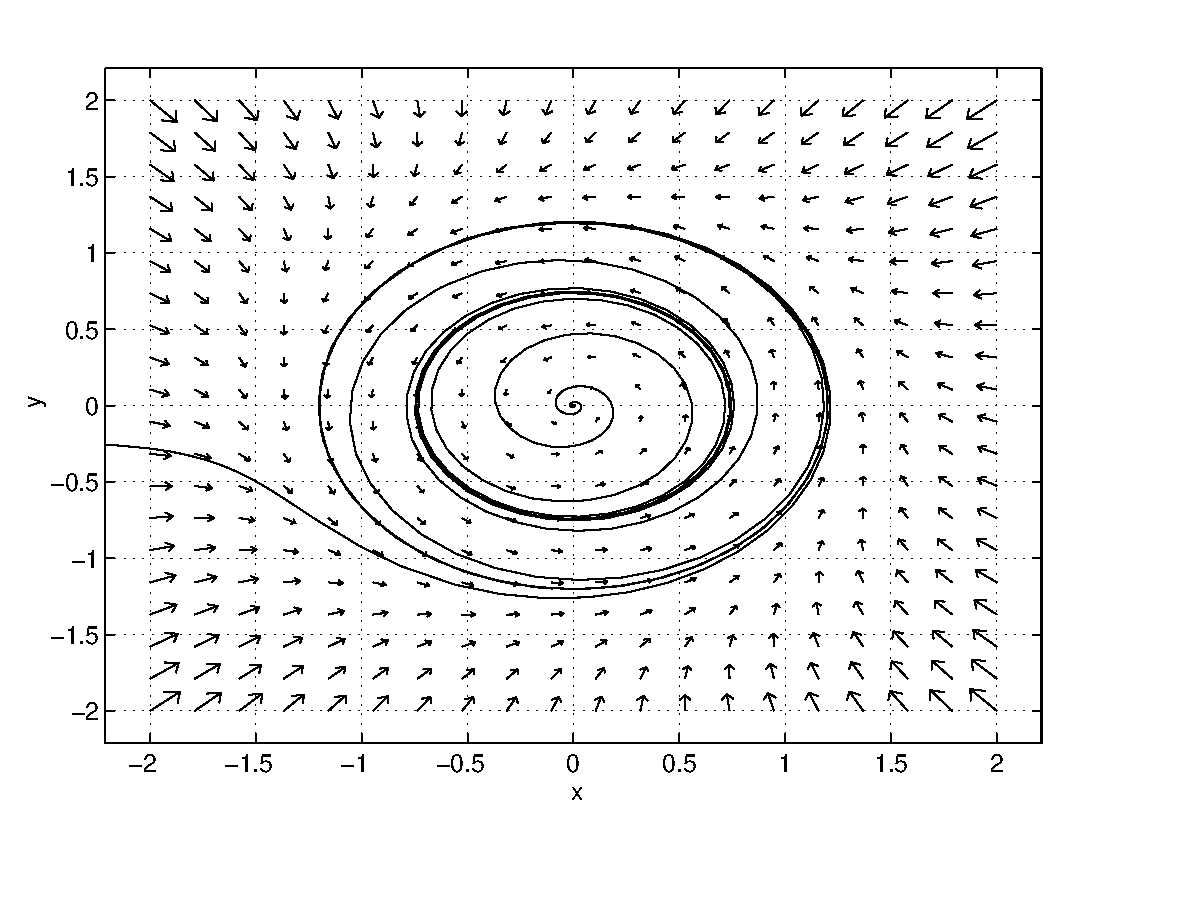
\psfig{file=figures/pappa.eps,width=2.3in}
	   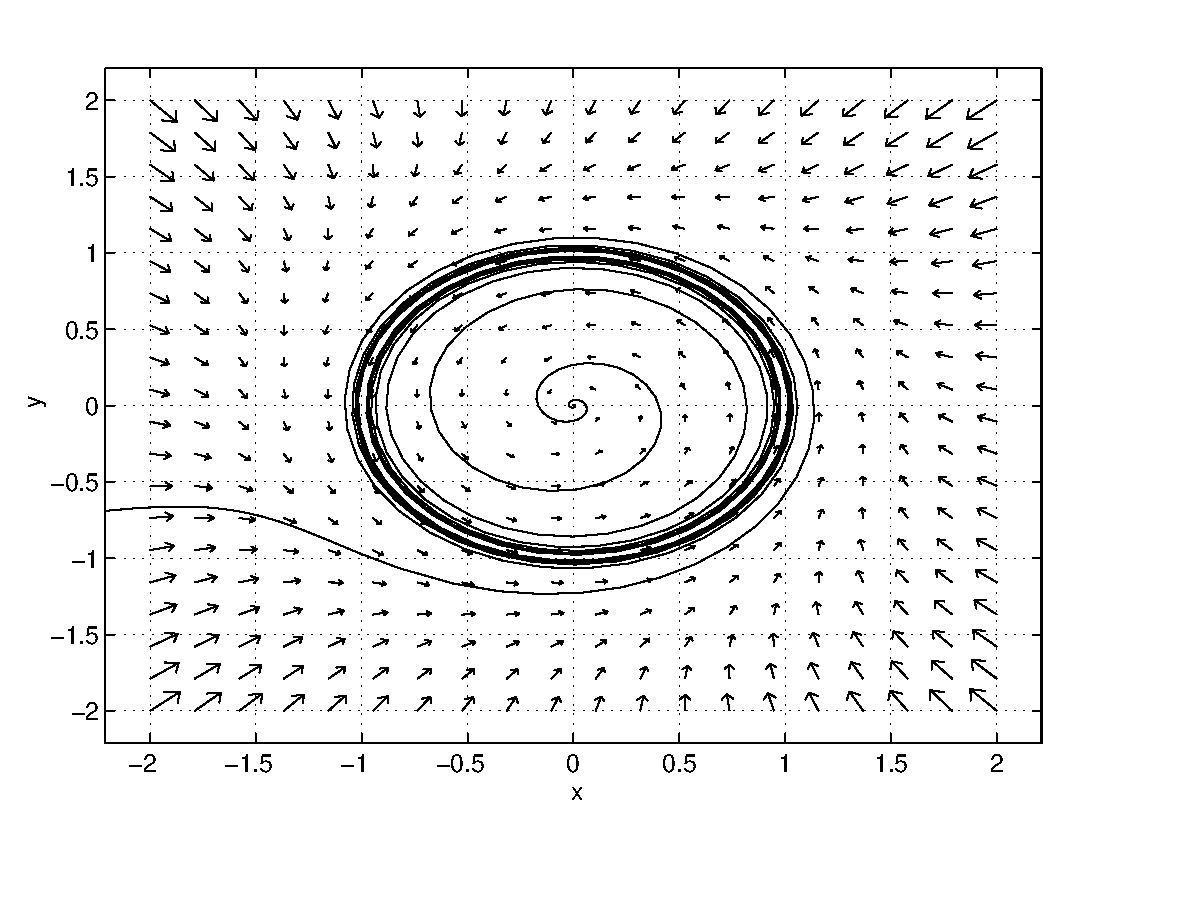
\psfig{file=figures/pappb.eps,width=2.3in}
	   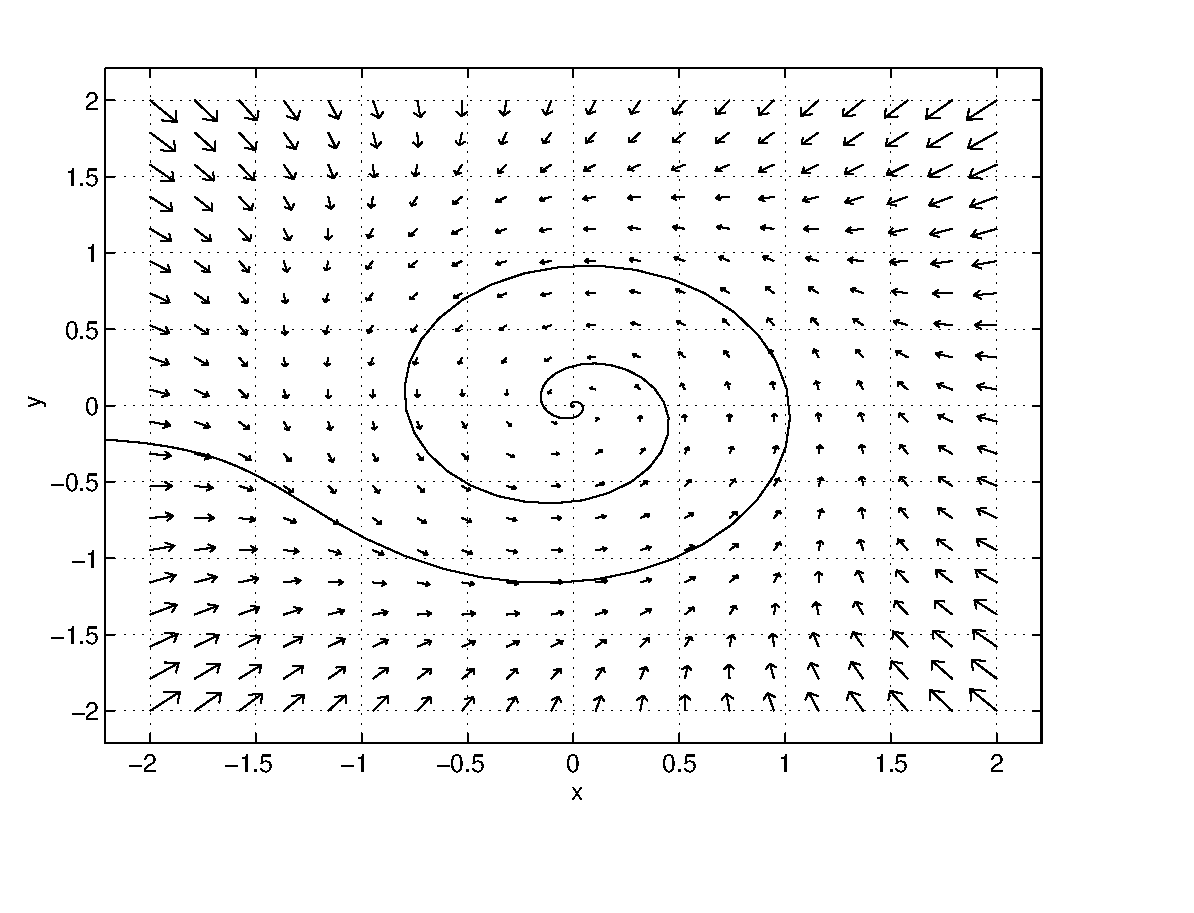
\psfig{file=figures/pappc.eps,width=2.3in}}
 	\vspace*{-0.2in}
	\hspace{0.3in} $\rho>0$  \hspace{1.9in} $\rho=0$
		\hspace{1.9in} $\rho<0$ 
           \caption{Phase portraits for \protect\Ref{e:papp}. 
Note that there are two limit cycles when $\rho>0$; one periodic solution 
when  $\rho=0$; and no periodic solutions when $\rho<0$.}
           \label{F:papp}
\end{figure}

In a sense, which we will not make precise, the annihilation of two
limit cycles in the plane through collision typically looks like the 
scenario shown in Figure~\ref{F:papp}.  



\subsection*{Saddle--Saddle Connections: Heteroclinic Trajectories}
\index{saddle-saddle connection}

In Section~\ref{S:bifurcation} we discussed the consequences of having a 
single trajectory connect a saddle point to itself.  As we have seen these 
homoclinic trajectories lead to the disappearance of a limit cycle.

When a single planar trajectory connects two different saddle points, the 
stable orbit of one saddle must become the unstable orbit of the other 
saddle.  This connecting trajectory is called a {\em heteroclinic\/} 
trajectory.\index{trajectory!heteroclinic}

We begin our discussion of heteroclinic connections with a simple example:
\begin{equation*} \label{e:hetero}
\begin{array}{rcl}
\dot{x} & = &  x^2-x  \\
\dot{y} & = &  y(0.5-x) + \rho x.
\end{array}
\end{equation*}
When $\rho=0$ the only equilibria of these equations are $(0,0)$ and 
$(1,0)$.  Note that when $y=0$ it follows that $\dot{y}=0$.  Hence
the $x$-axis is an invariant line for the dynamics of this equation. 
Moreover, a short calculation shows that both of these equilibria are 
saddle points and that the $x$-axis is the stable orbit for $(0,0)$
and the unstable orbit\index{unstable!orbit} for $(1,0)$.  
It follows that the line segment 
$(0,1)$ on the $x$-axis is a single trajectory that connects the two
equilibria.  This is an example of a heteroclinic trajectory. See
Figure~\ref{F:hetero}.  The time series for the heteroclinic trajectory 
is given in Figure~\ref{F:heteroT}.  Note the similarity to the time 
series in Figure~\ref{F:pp1dt} of the one dimensional equation 
\Ref{e:1dexample} discussed in the introduction to Chapter~\ref{C:NPS}. (In 
that example the trajectory connected $0$ in negative time to $1$ in positive
time, while in the present example the heteroclinic trajectory connects
$1$ in negative time to $0$ in positive time.)

\begin{figure}[htb]
           \centerline{%
	   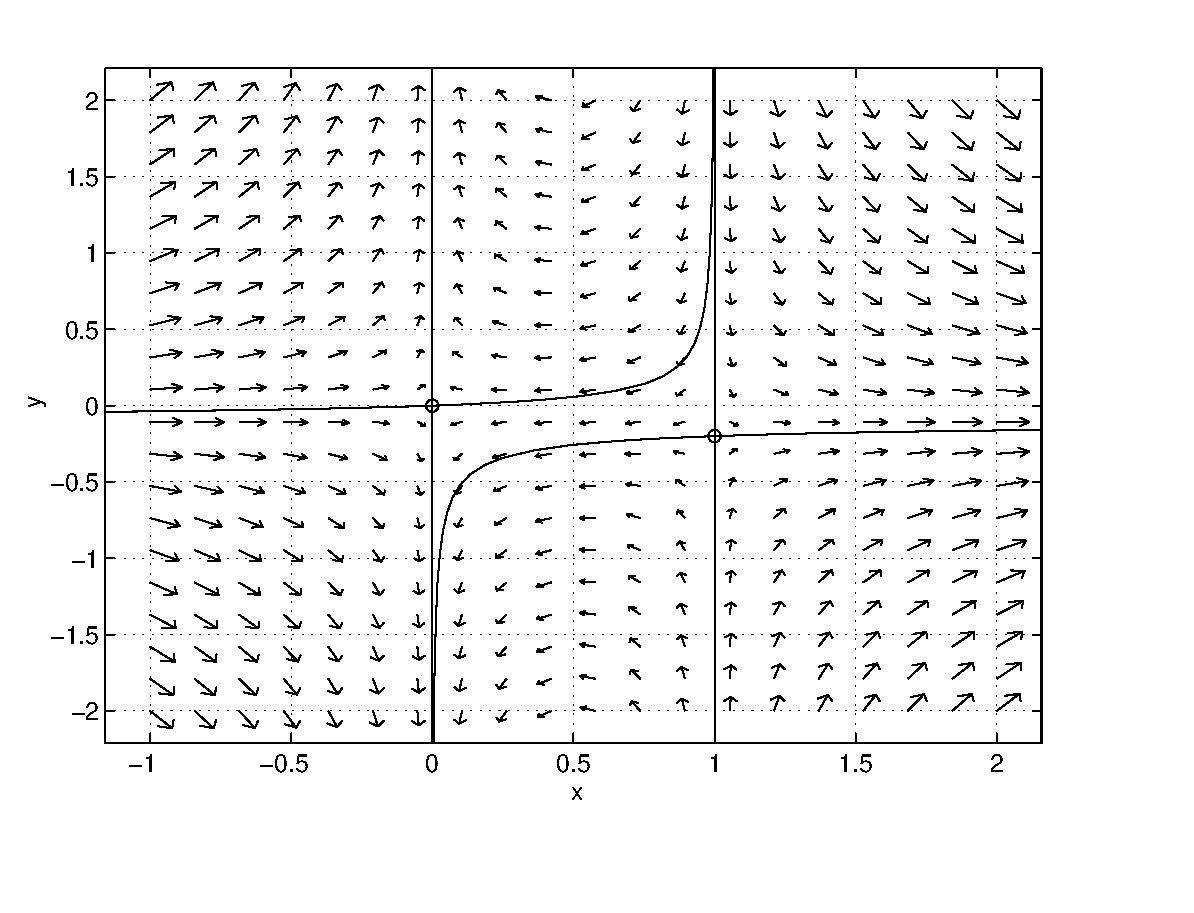
\psfig{file=figures/heteroa.eps,width=2.3in}
	   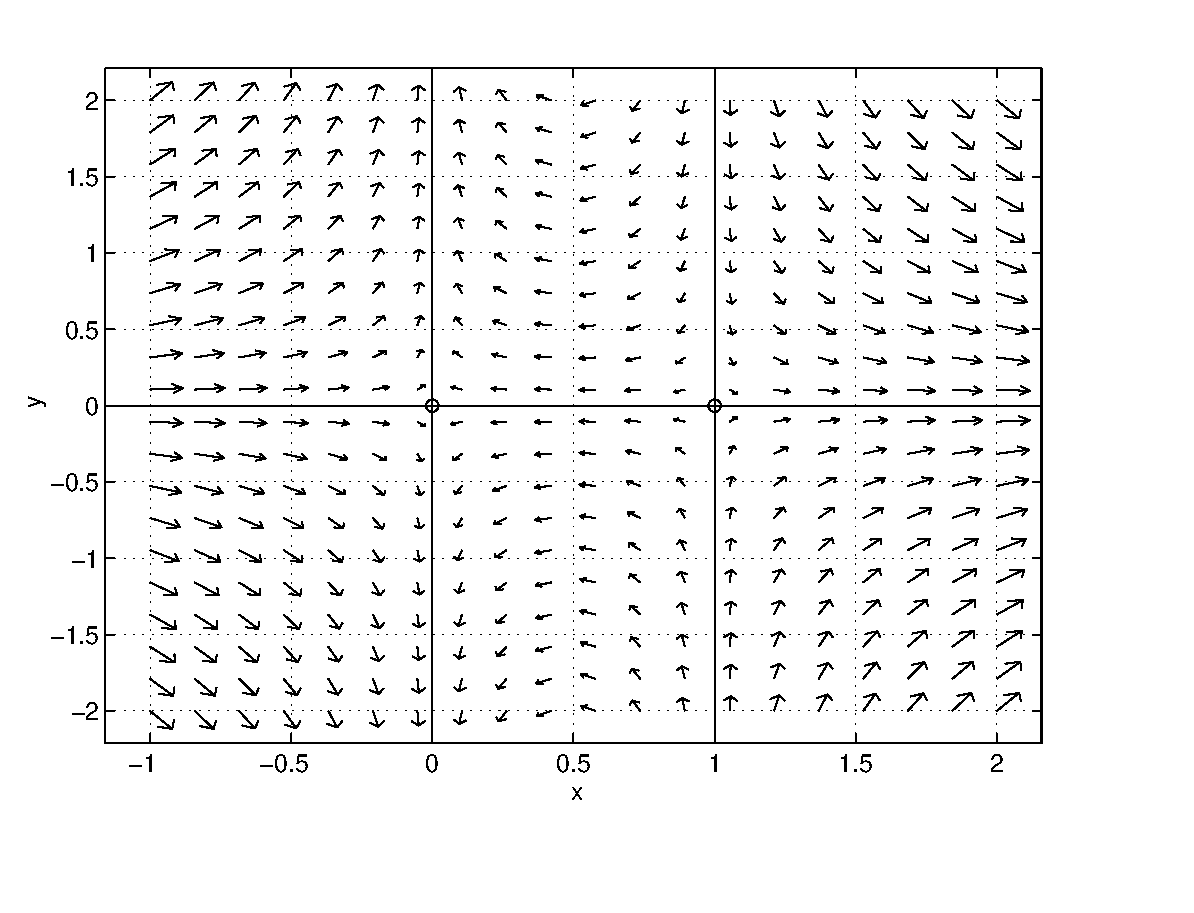
\psfig{file=figures/heterob.eps,width=2.3in}
	   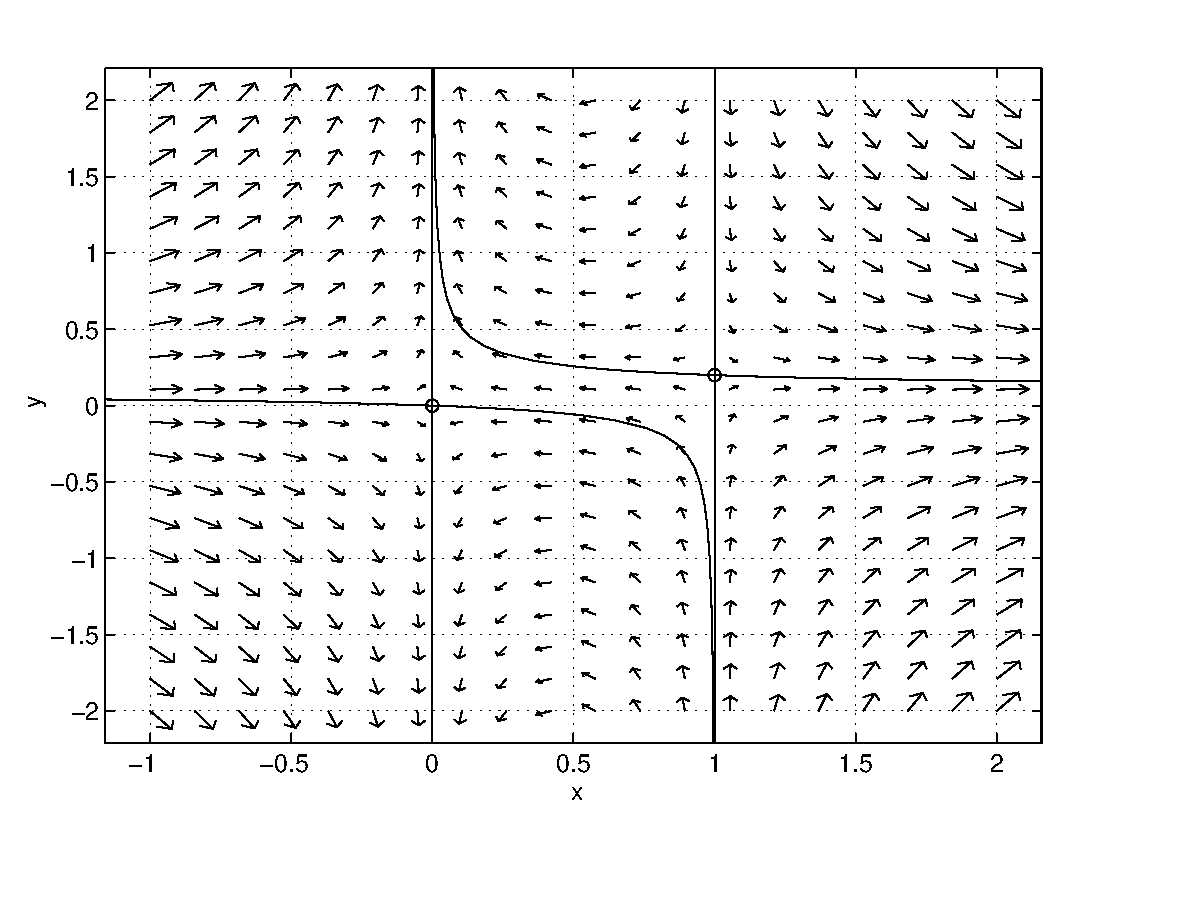
\psfig{file=figures/heteroc.eps,width=2.3in}}
 	\vspace*{-0.2in}
	\hspace{0.3in} $\rho=-0.1$  \hspace{1.7in} $\rho=0$
		\hspace{1.8in} $\rho=0.1$ 
           \caption{Phase portraits for \protect\Ref{e:hetero}. 
	Note the heteroclinic trajectory when $\rho=0$.}
           \label{F:hetero}
\end{figure}

\begin{figure}[htb]
           \centerline{%
	   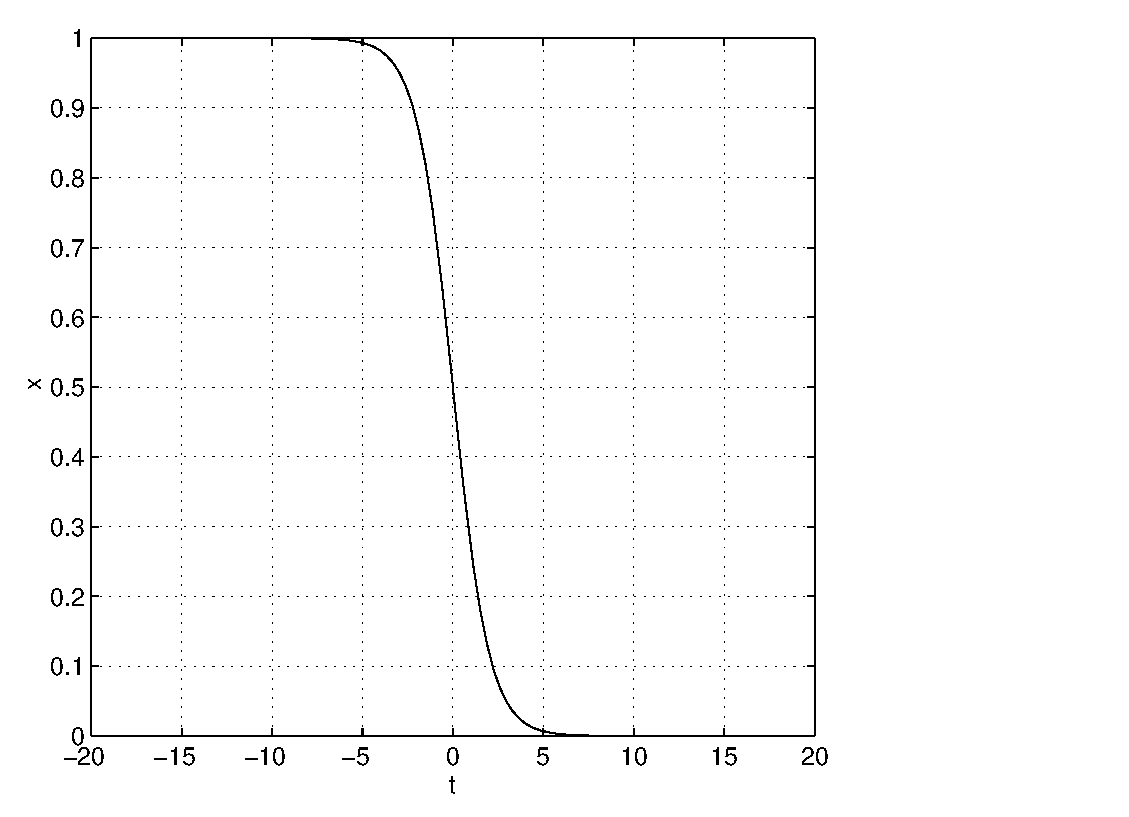
\psfig{file=figures/heteroT.eps,width=2.5in}}
           \caption{Time series for heteroclinic trajectory 
		in \protect\Ref{e:hetero} when $\rho=0$.}
           \label{F:heteroT}
\end{figure}

When $\rho\neq 0$ the $x$-axis is no longer invariant for the differential 
equation.  The two saddles remain --- but there is no longer a 
trajectory connecting them.  In Figure~\ref{F:hetero} we use 
{\sf pplane5}\index{stable!orbit!in {\sf pplane5}} 
\index{unstable!orbit!in {\sf pplane5}}
to plot the stable and unstable orbits when $\rho=\pm 0.1$.

From this figure we can see how the stable orbit of the origin swings 
through the saddle at $(1,0)$ as the parameter $\rho$ is varied.  This
is typical of the way that a heteroclinic trajectory appears and disappears 
as a parameter is varied.  The fleeting existence of a heteroclinic trajectory
shows how the global fate of stable and unstable orbits emanating from a 
saddle point can change in a drastic fashion. 


\subsection*{A Classification of One Parameter Bifurcations}

The following is a complete list of expected transitions between planar 
Morse-Smale systems of different types in systems with one parameter.
\index{Morse-Smale system}
\begin{itemize}
\item	Two equilibria coalesce and disappear in a saddle-node bifurcation.
\index{bifurcation!saddle-node}
\item	A single equilibrium changes from a spiral source to a spiral sink (or 
vice-versa) and spawns a limit cycle in a Hopf bifurcation.
\index{bifurcation!Hopf}
\item	Two limit cycles coalesce in a saddle-node bifurcation of 
periodic solutions\index{bifurcation!saddle-node!of periodic solutions}.
\item	Stable and unstable orbits from distinct saddle points
coalesce and form a heteroclinic trajectory\index{trajectory!heteroclinic}.
\item	Limit cycles grow until they touch a saddle and form a homoclinic 
trajectory\index{trajectory!homoclinic}.
\end{itemize}


\EXER

\CEXER

\begin{exercise} \label{c9.5.1}
Use {\sf pplane5} to analyze the phase portraits for the system
\begin{equation*}
\begin{array}{rcl}
\dot{x} & = & (-\rho+3(0.5x^2+y^2)-(x^2+y^2)^2)x-2y \\
\dot{y} & = & (-\rho+3(x^2+y^2)-(1.3x^2+y^2)^2)y+x
\end{array}
\end{equation*}
for $\rho=0.7$ and $\rho=1.1$ on the square $-2\leq x,y\leq 2$.  Is there 
a bifurcation between these two values of $\rho$?  If so, what kind of 
bifurcation is it and what is the bifurcation value of $\rho$ to within 
$\pm 0.02$?
\end{exercise}

\noindent In Exercises~\ref{c9.6.2a} -- \ref{c9.6.2c}, consider the system 
of differential equations \Ref{E:homo2}
\begin{equation*}  \label{E:homo2}
\begin{array}{rcl}
\dot{x} & = & -y + \rho x + 0.1 x^2 - 0.5 y^5 \\
\dot{y} & = & x +\rho y + 0.1 y^3 - x^4
\end{array}
\end{equation*}
in the square $-1.5\leq x,y\leq 1.5$.
\begin{exercise} \label{c9.6.2a}
Verify numerically that \Ref{E:homo2} appears to have a limit cycle for 
$\rho=-0.02$.
\end{exercise} 
\begin{exercise} \label{c9.6.2b}
Verify numerically that \Ref{E:homo2} does not appear to have a limit cycle 
when $\rho=-0.03$.
\end{exercise} 
\begin{exercise} \label{c9.6.2c}
Determine numerically to two significant figures, the value of $\rho$
where \Ref{E:homo2} has a homoclinic bifurcation. 
\end{exercise} 

\noindent In Exercises~\ref{c9.6.3a} -- \ref{c9.6.3b}, consider the system 
of differential equations \Ref{E:infinity}.
\begin{equation*}  \label{E:infinity}
\begin{array}{rcl}
\dot{x} & = & y \\
\dot{y} & = & -x +\rho y + \frac{1}{2}\cos(x)y
\end{array}
\end{equation*}
\begin{exercise} \label{c9.6.3a}
How many periodic solutions does \Ref{E:infinity} appear to have 
when $\rho=0$?  Be careful when answering this question.  First use 
{\sf pplane5} to determine the number of limit cycles on the square 
$-\ell \leq x,y \leq\ell$ when $\ell=2$.  Then compute with $\ell=10$ and 
$\ell=40$.
\end{exercise}
\begin{exercise} \label{c9.6.3b}
Find the number of limit cycles to \Ref{E:infinity} on the square 
with $\ell=7$ when $\rho=0.06$ and when $\rho=0.07$.  Has a bifurcation
 occurred between these two values of $\rho$ and, if so, what kind of 
bifurcation?
\end{exercise}

\noindent In Exercises~\ref{c9.6.4a} -- \ref{c9.6.4c}, consider the system 
of differential equations \Ref{E:twoeq}
\begin{equation*}  \label{E:twoeq}
\begin{array}{rcl}
\dot{x} & = & y - x + (x-\rho)^2 \\
\dot{y} & = & y - x^3 +3x
\end{array}
\end{equation*}
in the square $-5 \leq x,y \leq 5$.
\begin{exercise} \label{c9.6.4a}
How many equilibria does \Ref{E:twoeq} have in this square when 
$\rho=1.7$ and of what type are they?  This question can be answered either 
numerically using {\sf pplane5} (easy) or analytically (more difficult, but 
possible).
\end{exercise}
\begin{exercise} \label{c9.6.4b}
What type of bifurcation occurs in \Ref{E:twoeq} as $\rho$ is varied
from $\rho=1.7$ to $\rho=1.85$?
\end{exercise}
\begin{exercise} \label{c9.6.4c}
What type of bifurcation occurs in \Ref{E:twoeq} as $\rho$ is varied
from $\rho=1.85$ to $\rho=2.1$?
\end{exercise}

\begin{exercise} \label{c9.6.6}
Embed system \Ref{c8.4.5a} of Chapter~\ref{C:NPS} in the family of systems of 
differential equations 
\begin{equation} \label{E:eqn2}
\begin{array}{rcl}
\dot{x} & = & \rho x-y-3y^2+2.5xy\\
\dot{y} & = & x-3x^2+2x^2y.
\end{array}
\end{equation}
Find seven bifurcations that occur in \Ref{E:eqn2} as $\rho$ varies from 
$-0.1$ to $\rho=0.3$. 
\end{exercise}

\noindent In Exercises~\ref{c9.6.5a} -- \ref{c9.6.5c}, consider the system 
of differential equations \Ref{E:saddleconn}.
\begin{equation*}  \label{E:saddleconn}
\begin{array}{rcl}
\dot{x} & = & y  \\
\dot{y} & = & -x - 0.1y + x^3 + \rho x^2.
\end{array}
\end{equation*}
\begin{exercise} \label{c9.6.5a}
How many equilibria does \Ref{E:saddleconn} have for each value of 
$\rho$ and of what type are they?  
\end{exercise}
\begin{exercise} \label{c9.6.5b}
How many bifurcations occur in \Ref{E:saddleconn} as $\rho$ is 
varied from $\rho=0.1$ to $\rho=0.2$?
\end{exercise}
\begin{exercise} \label{c9.6.5c}
What types of bifurcation occur in \Ref{E:saddleconn} as $\rho$ is 
varied from $\rho=0.1$ to $\rho=0.2$?
\end{exercise}



\end{document}
